Гравитационное линзирование -- это отклонение  траектории света от прямолинейной в гравитационном поле массивных объектов. Выделяют три класса этого явления.

\begin{itemize}
    \item Сильное гравитационное линзирование, вызывающее легко различимые искажения, такие как кольцо или крест Эйнштейна, дуги и множественные изображения.
    \item Слабое гравитацонное линзирование, вызывающее слабое искажение источников, которые находятся позади линзы. Его можно зафиксировать только после статистического анализа объектов фона, что позволяет найти небольшое согласованное искажение их изображений. Проявляется в небольшом растяжении изображения перпендикулярно направлению к центру линзы.
    \item Микролинзирование, которое не вызывает видимых искажений формы, но может временно увеличивать или уменьшать количество света от источника. Более подробно микролинзирование описано в Главе \ref{ch:micro}.
\end{itemize}

Здесь и далее речь пойдет об эффекте сильного линзирования. Большая часть информации в данном разделе подробно представлена в книге (\cite{gravlensbook}). В рамках общей теории относительности можно показать, что в гравитационном поле точечного массивного тела (линзы) с ньютоновским потенциалом $\Phi$ угол отклонения светового луча равен

\begin{equation}\label{eq:angle}
%\hat
{\alpha}=\frac{2}{c^{2}} \int_{-\infty}^{+\infty} \vec{\nabla}_{\perp} \Phi \ \mathrm{d} z,
\end{equation}

\noindent где $z$ - координата вдоль невозмущённой траектории распространения света (\cite{narbart}, \cite{gl_all}). При этом предполагается, что $\Phi/c^2 \ll 1$, что выполняется практически всегда: например, для самых массивно гравитационно связанных объектов во Вселенной -- скоплений галактик --  $|\Phi|/c^2 \sim 10^{-4} \ll 1$. Это же условие обеспечивает малость углов: при сильном линзировании углы отклонения света порядка угловых секунд. Из того, что $\Phi$ не зависит от массы тела, попавшего в гравитационное поле, следует, что все фотоны отклоняются на один и тот же угол. Таким образом, сильное гравитационное линзирование ахроматично, то есть не зависит от длины волны. 
%Для точечной линзы $\Phi=-\frac{G M}{r}$, где $M$ - её масса, а значит, что углы отклонения массивом таких линз могут быть сложены по принципу суперпозиции. 

Непосредственно преломление происходит на очень коротком участке траетории света. В реалистичных моделях линз, в которых масса, вызывающая линзирование, распределена трёхмерным образом, используется приближение плоских линз по аналогии с геометрической оптикой. Это всегда оправдано: характерные размеры самого большого объекта, который может быть линзой, - скопления галактик - порядка 1 Мпк, в то время как продольные расстояния между объектами системы порядка 100-1000 Мпк. Типичная гравитационно-линзированная система изображена на Рисунке \ref{fig:gravlensfig}. 

\begin{figure}[H]
    \centering
	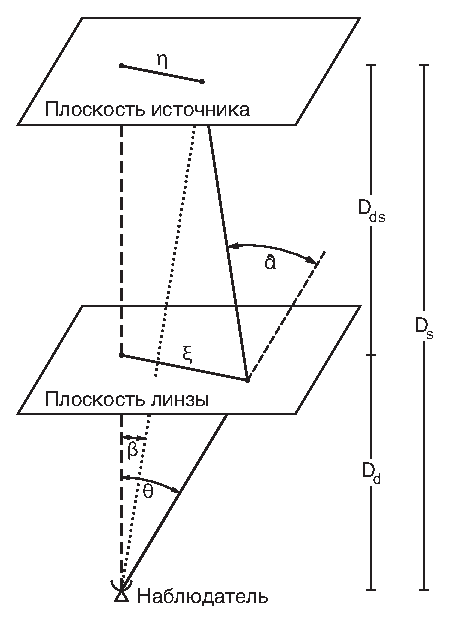
\includegraphics[scale=1.0]{pics/gr-lens-syst.eps}
	\caption{Типичная гравитационно линзированная система (\cite{gravlensbook}). Здесь $\beta$ и $\theta$ - углы между оптической осью (пунктирная линия) и источником и его изображением соответственно, $\hat{\alpha}$ - угол отклонения светового луча, $\eta$ и $\xi$ - расстояния от оптической оси до источника и его изображения соответственно,  $D_d$ - расстояние между наблюдателем и плоскостью линзы,$ D_{ds}$ - между плоскостями линзы и источника, $D_s$ - между наблюдателем и источником. Следует отметить, что в общем случае, $D_s \neq D_d + D_{ds}$.}
	\label{fig:gravlensfig}
\end{figure} 

Углами $\boldsymbol{\beta}$ и $\boldsymbol{\theta}$ (двумерными векторами в соответствующих плоскостях) задаются положения источника света и его изображения соответственно. Уравнение линзы, описывающее отображение из плоскости источника на плоскость линзы:

\begin{equation}\label{eq:lenseq}
\boldsymbol{\beta} = \boldsymbol{\theta} -  {\alpha}(\boldsymbol{\theta}) = \boldsymbol{\theta} - \frac{D_{ds}}{D_s} \hat{\alpha}(D_d\boldsymbol{\theta})
\end{equation}

\noindent где $\alpha(\boldsymbol{\theta})$ - угол между положениями источника и его наблюдаемого изображения в плоскости линзы, $\hat{\alpha}(\boldsymbol{\theta})$ - угол отклонения светового луча, $D_d$, $D_s$ и $D_{ds}$ - расстояния от наблюдателя до плоскости линзы, до источника и между плоскостями линзы и источника соответственно (см. Рис. \ref{fig:gravlensfig}). Также вводятся следующие величины: линзирующий гравитационный потенциал $\Psi(\boldsymbol{\theta})$ такой, что

\begin{equation}\label{eq:nablapsi}
\alpha(\boldsymbol{\theta}) = \nabla \Psi(\boldsymbol{\theta}),
\end{equation}

\noindent и безразмерная поверхностная плотность масс в линзе $\kappa$ (\textit{convergence}), определяемая условием

\begin{equation}\label{eq:nabla2psi}
\kappa({\boldsymbol{\theta}}) = \frac{1}{2}\nabla^2 \Psi(\boldsymbol{\theta}),
\end{equation}

Пусть масса линзы распределена в пространстве по закону $\rho(D_d \boldsymbol{\theta}, z)$, где $z$ - координата вдоль оптической оси. \textit{Поверхностная плотность} вещества в линзе задаётся следующим соотношением:

\begin{equation}\label{eq:sigmasurf}
\Sigma(D_d \boldsymbol{\theta})=\int \rho(D_d \boldsymbol{\theta}, z) \mathrm{d} z
\end{equation}

С учётом этого для $\kappa$ также верно соотношение

\begin{equation}\label{eq:convergence}
\kappa = \frac{\Sigma(D_d \boldsymbol{\theta})}{\Sigma_{crit}}, \ \ \ \ \  \textrm{где} \ \ \ \ \ \ \Sigma_{crit}=\frac{c^{2}}{4 \pi G} \frac{D_{\mathrm{s}}}{D_{\mathrm{d}} D_{\mathrm{ds}}},
\end{equation}

\noindent $c$ - скорость света, $G$ - гравитационная постоянная. По порядку величины $\Sigma_{crit} \sim 1 \ \textrm{г/см}^2$. Радиус такой окружности в плоскости линзы, плотность внутри которой равна критической, называется \textit{радиусом Эйнштейна}. Обычно он выражается в угловых единицах: 

\begin{equation}\label{eq:r_ein}
\theta_{E}=\sqrt{\frac{4 G M}{c^{2}} \frac{D_{d s}}{D_{d} D_{s}}},
\end{equation}
где $M$ - масса линзы. Эта величина характеризует масштабы гравитационного линзирования и является основной шкалой расстояний при описании этого явления.

В терминах линейной алгебры гравитационное линзирование можно описать как отображение плоскости источника на плоскость линзы, которое задаётся следующей матрицей:

\begin{equation}
\mathcal{A}(\boldsymbol{\theta})=\frac{\partial \boldsymbol{\beta}}{\partial \boldsymbol{\theta}}=\left(\delta_{i j}-\frac{\partial^{2} \Psi(\boldsymbol{\theta})}{\partial \theta_{i} \partial \theta_{j}}\right)=\left(\begin{array}{cc}{1-\kappa-\gamma_{1}} & {-\gamma_{2}} \\ {-\gamma_{2}} & {1-\kappa+\gamma_{1}}\end{array}\right)
\end{equation}

Безразмерная плотность  $\kappa$ отвечает за изотропное изменение линейных размеров изображения (увеличение или уменьшение), сдвиг (\textit{shear}) $\gamma=(\gamma_1,\gamma_2)$ характеризует анизотропное искажение формы изображений. Усиление изображения обратно пропорционально определителю этой матрицы (то есть якобиану этого отображения):

\begin{equation}\label{eq:magnification}
\mu=\frac{1}{\operatorname{det} \mathcal{A}} =  \frac{1}{(1-\kappa)^2-|\gamma|^2}
\end{equation}

Возможно существование некоторого множества точек, для которых выполняется соотношение $\operatorname{det} \mathcal{A}=0$, в которых усиление \textit{точечного} источника формально бесконечно. Кривая, образуемая этими точками, называется каустикой, а её образ в плоскости линзы – критической кривой. В реальности бесконечных усилений не наблюдается из-за неточечности источников, размер которых и ограничивает значение усиления. Источники, находящиеся по разные стороны от каустик, линзируются принципиально по-разному, чему уделено большое внимание как при изучении сильного гравитационного линзирования (\cite{blandfordnarayan1986}, \cite{narayanwallington1992}), так и микролинзирования (\cite{wambsganss1992-microlens}).

%https://arxiv.org/ftp/arxiv/papers/1604/1604.06351.pdf
 
%На Рисунке \ref{fig:caustics} видно, как ведёт себя изображение компактного источника при пересечении им складки \textit{(fold)} или излома \textit{(cusp)} каустики.
 
%\begin{figure}[H]
%    \centering
%	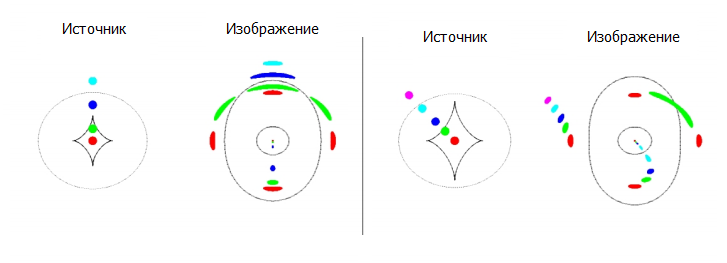
\includegraphics[scale=0.8]{pics/caust_intro.png}
%	\caption{Поведение изображения компактного источника при пересечении им излома (левая панель) или складки (правая панель) каустики  (\cite{narbart}). Также для иллюстрации изменения масштабов изображения нарисованы критические кривые в плоскости линзы. \label{fig:caustics}}
%\end{figure}


